\chapter{Data Pre Processing}
\section{Data}
The attribute can be everything , we can give order and distinct them. The biggest difference is between discrete or continuous attribute, the continuous can be transformed or we can represent them with floating point variables.
The dataset are also divided in record, graph or ordered. The record could be Tables,document or transaction data.

The data can have a lot of quality problems due to their origins like noise or outlier, missing values or duplicate data. The action to perform is the \textbf{data cleaning}

\section{Distance}
We can confront two data object with the similarity or dissimilarity, to calculate we have a lot of different distance that we can compute.

The \textbf{euclidean distance }is the simplest one, standardization might be applied, if scales differ:
\begin{center}
    $d(x,y) = \sqrt{\sum\limits_{k=1}^n (x_k - y_k)^2 }$
\end{center}

\textbf{Minkowsky distance} is a generalization of Euclidean Distance:

\begin{center}
    $d(x,y) = (\sum\limits_{k=1}^n | x_k - y_k |^r )^{1/r} $
\end{center}
There is also the \textbf{Manhattan} $d(x,y) = |x_1 - x_2| + |y_1 -y_2| $ and a lot of other.

\textbf{Mahalanobis distance} measures the distance between two points with respect to a probability distribution with covariance matrix S and also  is thus unitless, scale- invariant, and takes into account the correlations of the data set
\begin{center}
    $ d(x,y,S) = \sqrt{(x-y)^T S^{-1} (x-y)}$
\end{center}
\section{Data pre-processing}
\textbf{Data aggregation} is about combining two or more attributes (or objects) into a single attribute (or object) to reduce the data, change the scale or have more stable data\\
\textbf{Data reduction} is about generates a reduced representation of the dataset with similar analytical results this could be done with sampling, discretization or with feature selection and creation\\
\textbf{Sampling} is the main technique employed for data selection and it is often used for both the preliminary investigation of the data and the final data analysis because processing the entire set of data of interest might be too expensive or time consuming, the key principle for effective sampling is that a good sample will always work like the dataset and can approximately have the same property. There are several types of sampling like the simple random sampling or the stratified one that split the data into several partition and then draw samples from each partition.

We can have a problem called \textbf{curse of dimensionality} because when feature dimensionality increases, data becomes increasingly sparse in the space that it occupies and the definitions of density and distance between points, which is critical for clustering and outlier detection, become less meaningful.

One method is called recursive feature elimination that assigns weights to features and then selects features by recursively considering smaller and smaller sets of features.  First, the estimator is trained on the initial set of features and the importance of each feature is obtained, the least important features are pruned from current set of features. That procedure is recursively repeated on the pruned set until the
desired number of features to select is eventually reached

Indeed we have to find a way to reduce dimensionality of the data deleting redundant and irrelevant features. Other method could be assign weight to features or selects features by recursively considering smaller sets. More important are the automatic feature selection like \textbf{PCA} or \textbf{SVD}.
\section{Data Engineering}
Feature Engineering is the act of extracting features from raw data and transforming them to more useful, from a lot to few. Basic types of feature engineering include:
\begin{itemize}
    \item Data transformation
    \item Normalization
    \item Discretization
    \item Binarization
\end{itemize}
\textbf{Data transformation} is the process of converting data from one format to another and it is useful because non numerical data is difficult to analyze if not transformed into numerical and to capture important information or to better visualize the data

\textbf{Discretization }is the process of converting a continuous attribute into an ordinal attribute: A potentially infinite number of values are mapped into a small number of categories, for example {high, medium, low} or binary attributes or one-hot encoding. One hot encoding use a group of bits to represent possible categories, similar speech for Dummy coding and Effect coding.

\textbf{Normalization} refers to various techniques to adjust to differences among attributes in terms of mean, variance, range It is performed with the attribute transform that is is a function that maps the entire set of values of a given attribute to a new set of replacement values such that each old value can be identified with one of the new values. There are a lot of different normalization.
\begin{center}
    Min-max normalization  $x'= \dfrac{x-x_{min}}{x_{max} - x_{min}}$
\end{center}
This one rescale the functions and is a unity based normalization, is a technique that bring all values into the range of [0,1] retains the shape of the distribution.
\begin{figure}[H]
    \centering
    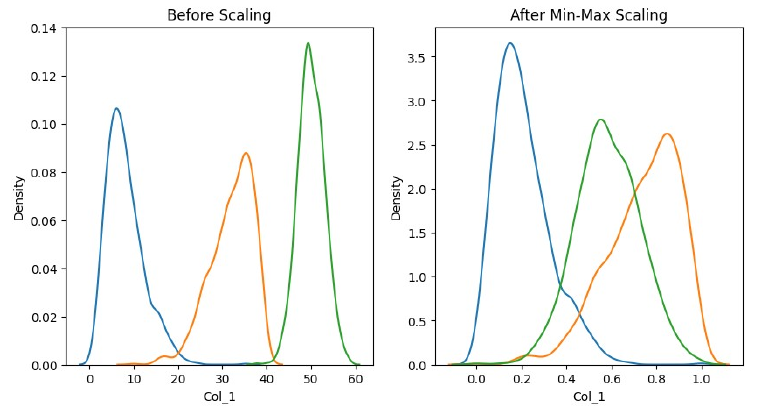
\includegraphics[scale=0.5]{images/Data pre-process/MINMAX.png}
    \caption{Example of Min max normalization}
    \label{fig:enter-label}
\end{figure}

\begin{center}
    Standardization  $x'= \dfrac{x- \mu}{\sigma}$
\end{center}

It is a bit different from the previous one because it is not bounded to a certain range and t is used when we want to ensure zero mean and unit standard deviation
\begin{figure}[H]
    \centering
    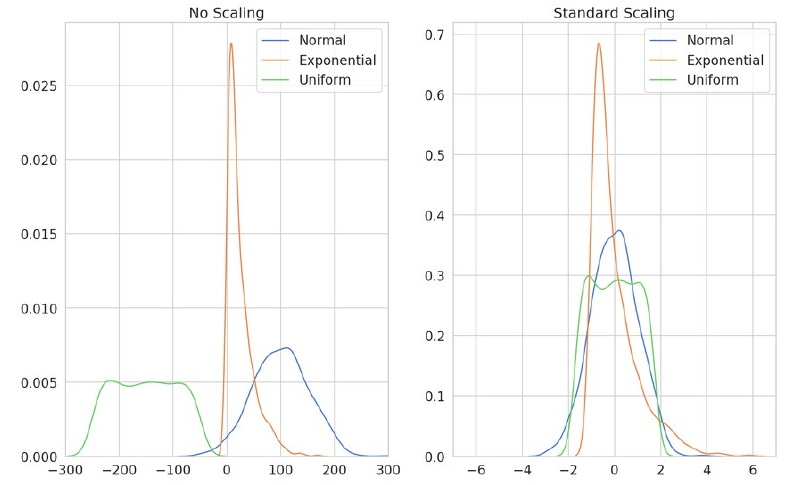
\includegraphics[scale=0.5]{images/Data pre-process/Standard.png}
    \caption{Example of standardization}
    \label{fig:enter-label}
\end{figure}

\section{Data preparation for document data}

A document might be modeled in different ways and the choice heavily affects the quality of the mining result, often document are represented as a set of features and might represent set of characters, word, term, concept. The document preprocessing is the activity to generate a structured data representation of document data and includes 5 sequential steps:
\begin{itemize}
    \item Document splitting
    \item Tokenization
    \item Case normalization
    \item Stopword removal
    \item Stemming
\end{itemize}
Document splitting is based on the data analytics goal, documents can be split into sentences, paragraphs, or analyzed in their entire content.

Case normalization is the process of breaking text into sentences or text into tokens but it is language-dependent and this step converts each token to completely upper-case or lower-case characters, then it is appropriate to eliminate the stop word: Preposition, article, conjunctions.

But not for each algorithms the words are able to be processed so they can be transformed into numbers or other type of data. Documents are represented by feature vectors with a feature that represent an entity without internal structure.

\textbf{Bag of words} are the representation for the words in a document and every word is considered as a feature, where the dimension is equal to the number of different words and there is a set of weights, one for each distinct word

\begin{figure}[H]
    \centering
    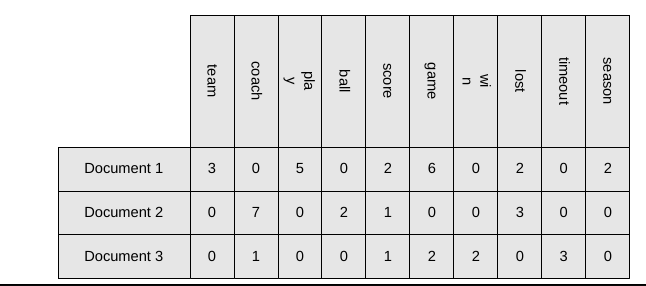
\includegraphics[scale=0.6]{images/Data pre-process/Word-bag.png}
    \caption{Example of bag of word}
    \label{fig:enter-label}
\end{figure}

The weighting schemes can be:
\begin{itemize}
    \item  Binary
        \begin{itemize}
            \item One, if the corresponding word is present in the document
            \item Zero, otherwise
            \item Occurrences of all words have the same importance
        \end{itemize}
    \item Simple document frequency
        \begin{itemize}
            \item The number of times in which the corresponding word occurs in the document
            \item Most frequent words are not always representative of the document content
        \end{itemize}
    \item Term frequency inverse document frequency (tf-idf)
        \begin{itemize}
            \item Tf-idf of term $t$ in document d of collection $D$ (consisting of m documents)
            \item Terms occurring frequently in a single document but rarely in the whole collection are preferred
            \item  tf-idf(t)$=   freq(t,d)*log(\dfrac{m}{freq(t,D)} ) $
        \end{itemize}
\end{itemize}


 
